\documentclass[11pt,a4paper]{article}
\usepackage[spanish,es-nodecimaldot]{babel}	% Utilizar español
\usepackage[utf8]{inputenc}					% Caracteres UTF-8
\usepackage{graphicx}						% Imagenes
\usepackage[hidelinks]{hyperref}			% Poner enlaces sin marcarlos en rojo
\usepackage{fancyhdr}						% Modificar encabezados y pies de pagina
\usepackage{float}							% Insertar figuras
\usepackage[textwidth=390pt]{geometry}		% Anchura de la pagina
\usepackage[nottoc]{tocbibind}				% Referencias (no incluir num pagina indice en Indice)
\usepackage{enumitem}						% Permitir enumerate con distintos simbolos
\usepackage[T1]{fontenc}					% Usar textsc en sections
\usepackage{amsmath}						% Símbolos matemáticos

% Comando para poner el nombre de la asignatura
\newcommand{\asignatura}{Aprendizaje Automático}
\newcommand{\autor}{Vladislav Nikolov Vasilev}

% Configuracion de encabezados y pies de pagina
\pagestyle{fancy}
\lhead{\autor{}}
\rhead{\asignatura{}}
\lfoot{Grado en Ingeniería Informática}
\cfoot{}
\rfoot{\thepage}
\renewcommand{\headrulewidth}{0.4pt}		% Linea cabeza de pagina
\renewcommand{\footrulewidth}{0.4pt}		% Linea pie de pagina

\begin{document}
\pagenumbering{gobble}

% Pagina de titulo
\begin{titlepage}

\begin{minipage}{\textwidth}

\centering

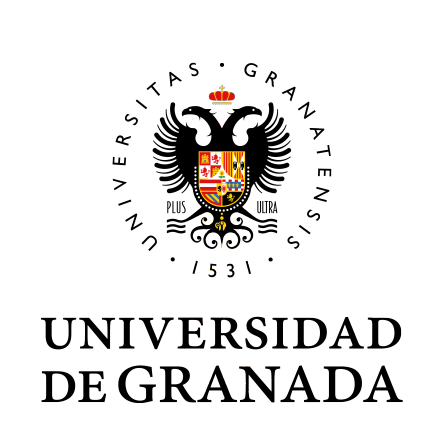
\includegraphics[scale=0.5]{img/ugr.png}\\

\textsc{\Large \asignatura{}\\[0.2cm]}
\textsc{GRADO EN INGENIERÍA INFORMÁTICA}\\[1cm]

\noindent\rule[-1ex]{\textwidth}{1pt}\\[1.5ex]
\textsc{{\Huge PRÁCTICA 3\\[0.5ex]}}
\textsc{{\Large Programación\\}}
\noindent\rule[-1ex]{\textwidth}{2pt}\\[3.5ex]

\end{minipage}

\vspace{0.5cm}

\begin{minipage}{\textwidth}

\centering

\textbf{Autor}\\ {\autor{}}\\[2.5ex]
\textbf{Rama}\\ {Computación y Sistemas Inteligentes}\\[2.5ex]
\vspace{0.3cm}


\includegraphics[scale=0.3]{img/etsiit.jpeg}

\vspace{0.7cm}
\textsc{Escuela Técnica Superior de Ingenierías Informática y de Telecomunicación}\\
\vspace{1cm}
\textsc{Curso 2018-2019}
\end{minipage}
\end{titlepage}

\pagenumbering{arabic}
\tableofcontents
\thispagestyle{empty}				% No usar estilo en la pagina de indice

\newpage

\setlength{\parskip}{1em}

\section{\textsc{Problema de Regresión}}

\subsection{Descripción del problema}

En este problema vamos a trabajar con el conjunto de datos \textit{Airfoil Self-Noise}, el cuál ha sido proporcionado por la NASA,
y contiene los resultados de haber realizado un conjunto de pruebas aerodinámicas y acústicas en un túnel de viento sobre perfiles
alares de dos y tres dimensiones.

El conjunto de datos está compuesto por 1503 filas y 6 columnas, los valores de las cuáles son todos números reales. Los datos de
las 5 primeras columnas se corresponden con los datos de entrada, y la última columna se corresponde con la información de salida.
A continuación se puede ver que representa cada uno de los atributos de forma ordenada:

\begin{enumerate}
	\item Frecuencia, medida en $Hz$.
	\item Ángulo de ataque (ángulo que forman la cuerda geométrica de un perfil alar con la dirección del aire incidente),
		  medida en grados.
	\item Longitud de la cuerda del perfil alar, medida en metros.
	\item Velocidad \textit{free-stream}, medida en metros por segundo. 
	\item Distancia de desplazamiento de succión, medida en metros.
	\item Nivel de presión sonora, medida en $dB$.
\end{enumerate}

\subsection{Análisis, particionado y preprocesado de los datos}

\newpage

\section{\textsc{Problema de Clasificación}}

\newpage

\begin{thebibliography}{5}

\bibitem{nombre-referencia}
Texto referencia
\\\url{https://url.referencia.com}

\end{thebibliography}

\end{document}

